\documentclass[12pt,a4paper]{article}
\usepackage{amsmath,amssymb,mathrsfs,tikz,times,pifont}
\usepackage{enumitem}
\newcommand\circitem[1]{%
\tikz[baseline=(char.base)]{
\node[circle,draw=gray, fill=red!55,
minimum size=1.2em,inner sep=0] (char) {#1};}}
\newcommand\boxitem[1]{%
\tikz[baseline=(char.base)]{
\node[fill=cyan,
minimum size=1.2em,inner sep=0] (char) {#1};}}
\setlist[enumerate,1]{label=\protect\circitem{\arabic*}}
\setlist[enumerate,2]{label=\protect\boxitem{\alph*}}
%%%::::::by chnini ameur :::::::%%%
\everymath{\displaystyle}
\usepackage[left=1cm,right=1cm,top=1cm,bottom=1.7cm]{geometry}
\usepackage[colorlinks=true, linkcolor=blue, urlcolor=blue, citecolor=blue]{hyperref}
\usepackage{array,multirow}
\usepackage[most]{tcolorbox}
\usepackage{varwidth}
\usepackage{float} %pour utiliser l'option [H] qui force l'image à apparaître exactement à l'endroit où elle est placée dans le code.
\usepackage{comment}
\tcbuselibrary{skins,hooks}
\usetikzlibrary{patterns}
%%%::::::by chnini ameur :::::::%%%
\newtcolorbox{exa}[2][]{enhanced,breakable,before skip=2mm,after skip=5mm,
colback=yellow!20!white,colframe=black!20!blue,boxrule=0.5mm,
attach boxed title to top left ={xshift=0.6cm,yshift*=1mm-\tcboxedtitleheight},
fonttitle=\bfseries,
title={#2},#1,
% varwidth boxed title*=-3cm,
boxed title style={frame code={
\path[fill=tcbcolback!30!black]
([yshift=-1mm,xshift=-1mm]frame.north west)
arc[start angle=0,end angle=180,radius=1mm]
([yshift=-1mm,xshift=1mm]frame.north east)
arc[start angle=180,end angle=0,radius=1mm];
\path[left color=tcbcolback!60!black,right color = tcbcolback!60!black,
middle color = tcbcolback!80!black]
([xshift=-2mm]frame.north west) -- ([xshift=2mm]frame.north east)
[rounded corners=1mm]-- ([xshift=1mm,yshift=-1mm]frame.north east)
-- (frame.south east) -- (frame.south west)
-- ([xshift=-1mm,yshift=-1mm]frame.north west)
[sharp corners]-- cycle;
},interior engine=empty,
},interior style={top color=yellow!5}}
%%%%%%%%%%%%%%%%%%%%%%%

\usepackage{fancyhdr}
\usepackage{eso-pic}         % Pour ajouter des éléments en arrière-plan
% Commande pour ajouter du texte en arrière-plan
\usepackage{tkz-tab}
\AddToShipoutPicture{
    \AtTextCenter{%
        \makebox[0pt]{\rotatebox{80}{\textcolor[gray]{0.7}{\fontsize{5cm}{5cm}\selectfont PGB}}}
    }
}
\usepackage{lastpage}
\fancyhf{}
\pagestyle{fancy}
\renewcommand{\footrulewidth}{1pt}
\renewcommand{\headrulewidth}{0pt}
\renewcommand{\footruleskip}{10pt}
\fancyfoot[R]{
\color{blue}\ding{45}\ \textbf{2024}
}
\fancyfoot[L]{
\color{blue}\ding{45}\ \textbf{Prof:M. BA}
}
\cfoot{\bf
\thepage /
\pageref{LastPage}}

% Définition de l'encadré adaptatif avec fond jaune
\newtcolorbox{resultbox}{
    colback=red!30, % Fond rouge clair
    colframe=black, % Bordure noire fine
    sharp corners, % Coins nets
    boxrule=0.5pt, % Contour léger
    boxsep=2pt, % Espacement interne
    left=5pt, right=5pt, top=2pt, bottom=2pt, % Marges internes
}

\begin{document}
\renewcommand{\arraystretch}{1.5}
\renewcommand{\arrayrulewidth}{1.2pt}
\begin{tikzpicture}[overlay,remember picture]
\node[draw=blue,line width=1.2pt,fill=purple,text=blue,inner sep=3mm,rounded corners,pattern=dots]at ([yshift=-2.5cm]current page.north) {\begingroup\setlength{\fboxsep}{0pt}\colorbox{white}{\begin{tabular}{|*1{>{\centering \arraybackslash}p{0.28\textwidth}} |*2{>{\centering \arraybackslash}p{0.2\textwidth}|} *1{>{\centering \arraybackslash}p{0.19\textwidth}|} }
\hline
\multicolumn{3}{|c|}{$\diamond$$\diamond$$\diamond$\ \textbf{Lycée de Dindéfélo}\ $\diamond$$\diamond$$\diamond$ }& \textbf{A.S. : 2024/2025} \\ \hline
\textbf{Matière: Mathématiques}& \textbf{Niveau : T}\textbf{S2} &\textbf{Date: 09/12/2024} & \textbf{Durée : 4 heures} \\ \hline
\multicolumn{4}{|c|}{\parbox[c]{10cm}{\begin{center}
\textbf{{\Large\sffamily Correction du devoir n$ ^{\circ} $ 2 Du 1$ ^\text{\bf er} $ Semestre}}
\end{center}}} \\ \hline
\end{tabular}}\endgroup};
\end{tikzpicture}
\vspace{3cm}

\section*{\underline{Exercice 1 :} 0,5 $\times $ 10 = 5 points}

\begin{enumerate}
    \item Déterminons une primitive $F$ de la fonction $f$ sur $I$.
    \begin{enumerate}
        \item $f(x) = (6x - 3)(4x^2 - 4x + 2)^3 \quad ; I = \mathbb{R}$ \textbf{(0,5pt)}
        
        $
        \begin{aligned}
        f(x) &= (6x - 3)(4x^2 - 4x + 2)^3\\
             &= 3(2x - 1)(4x^2 - 4x + 2)^3\\
             &= 3\times \dfrac{1}{4}(8x - 4)(4x^2 - 4x + 2)^3\\
             &= 3\times \dfrac{1}{4}(4x^2 - 4x + 2)'(4x^2 - 4x + 2)^3\\
             &=3\times \dfrac{1}{4}u'u^{3}
        \end{aligned}
        $

        $
        \begin{aligned}
        F(x) &=3\times \dfrac{1}{4}\times \dfrac{1}{4}u^{4} +k\\
             &= 3\times \dfrac{1}{4} \times \dfrac{1}{4} (4x^2 - 4x + 2)^4 +k\\
             &= \dfrac{3}{16} (4x^2 - 4x + 2)^4 +k\\
        \end{aligned}
        $        

\begin{resultbox}
    \[
    \mathbf{F(x) = \dfrac{3}{16} (4x^2 - 4x + 2)^4}+k
    \]
\end{resultbox}        
        
        \item $f(x) = \dfrac{\sin x}{\sqrt{3 + \cos x}} \quad ; I = \mathbb{R}$ \textbf{(0,5pt)}

$
        \begin{aligned}
        f(x) &= \dfrac{\sin x}{\sqrt{3 + \cos x}}\\
             &= \dfrac{-(3 + \cos x)'}{\sqrt{3 + \cos x}}\\
             &= \dfrac{-(u)'}{\sqrt{u}}\\
        \end{aligned}
        $

        $
        \begin{aligned}
        F(x) &= -2\sqrt{u}+k\\
             &= -2\sqrt{3 + \cos x} +k
        \end{aligned}
        $        

\begin{resultbox}
    \[
    \mathbf{F(x) = -2\sqrt{3 + \cos x} +k }
    \]
\end{resultbox}               
        
        \item $f(x) = 2\cos 3x - 3\sin 2x \quad ; I = \mathbb{R}$ \textbf{(0,5pt)}

$
        \begin{aligned}
        f(x) &= 2\cos 3x - 3\sin 2x\\
             &= 2 \times \cos (ax+b) - 3 \times \sin (ax+b)\\
        \end{aligned}
        $

        $
        \begin{aligned}
        F(x) &= 2 \times \dfrac{1}{a} \sin (ax+b) + 3 \times \dfrac{1}{a} \cos (ax+b)\\
             &= 2 \times \dfrac{1}{3} \sin (3x) + 3 \times \dfrac{1}{2} \cos (2x)\\ 
             &= \dfrac{2}{3} \sin (3x) + \dfrac{3}{2} \cos (2x)\\ 
        \end{aligned}
        $        

\begin{resultbox}
    \[
    \mathbf{F(x) = \dfrac{2}{3} \sin (3x) + \dfrac{3}{2} \cos (2x) +k }
    \]
\end{resultbox}     
        
        \item $f(x) = \dfrac{3x}{\sqrt{x^2 - 1}} + \sin x \sin 2x \quad ; I = ]-\infty; -1[$ \textbf{(0,5pt)}

$
        \begin{aligned}
        f(x) &= \dfrac{3x}{\sqrt{x^2 - 1}} + \sin x \sin 2x\\
             &= \dfrac{3x}{\sqrt{x^2 - 1}} + \sin x \times \cos x \times \sin x\\
             &= \dfrac{3x}{\sqrt{x^2 - 1}} + \cos x \times \sin^{2} x\\
             &= \dfrac{3}{2}\dfrac{(x^2 - 1)'}{\sqrt{x^2 - 1}} +\dfrac{1}{3} (\sin^{3} x)'\\
             &= \dfrac{3}{2}\dfrac{(u)'}{\sqrt{u}} +\dfrac{1}{n+1} (\sin^{n+1} x)'\\
        \end{aligned}
        $

        $
        \begin{aligned}
        F(x) &= \dfrac{3}{2}\times 2\sqrt{u} +\dfrac{1}{3} \sin^{3} x + k\\
             &= 3\sqrt{x^2 - 1} +\dfrac{1}{3} \sin^{3} x +k\\ 
        \end{aligned}
        $        

\begin{resultbox}
    \[
    \mathbf{F(x) = 3\sqrt{x^2 - 1} +\dfrac{1}{3} \sin^{3} x +k }
    \]
\end{resultbox}         
        
    \end{enumerate}
    \item Soit $k$ la fonction définie sur $\mathbb{R} \setminus \{-2\}$ par : $k(x) = \dfrac{3x - 2}{(x+2)^3}$.
    \begin{enumerate}
        \item Déterminons les $a$ et $b$ tels que $\forall x \in \mathbb{R} \setminus \{-2\}$, $k(x) = \dfrac{a}{(x+2)^2} + \dfrac{b}{(x+2)^3}$. \textbf{(0,5pt)}

        $
        \begin{aligned}
        k(x) &= \dfrac{a}{(x+2)^2} + \dfrac{b}{(x+2)^3}\\
             &= \dfrac{a(x+2)}{(x+2)^3} + \dfrac{b}{(x+2)^3}\\
             &= \dfrac{a(x+2)+b}{(x+2)^3}\\
             &= \dfrac{ax+2a+b}{(x+2)^3}\\
        \end{aligned}
        $        

Par indentification $3x - 2 = ax+2a+b$

        $
        \begin{aligned}
        3x - 2 = ax+2a+b & \implies \begin{cases} a = 3  \\ 2a+b = -2 \end{cases}\\
        								 & \implies \begin{cases} a = 3  \\ 6+b = -2 \end{cases}\\
        								 & \implies \begin{cases} a = 3  \\ b = -8 \end{cases}\\
        \end{aligned}
        $        

Donc  $k(x) = \dfrac{3}{(x+2)^2} + \dfrac{-8}{(x+2)^3}$

\begin{resultbox}
    \[
    \mathbf{k(x) = \dfrac{3}{(x+2)^2} + \dfrac{-8}{(x+2)^3} +c }
    \]
\end{resultbox}          
        
        \item Déduisons-en la primitive $K$ de $k$ qui prend la valeur 2 en -3. \textbf{(0,5pt)}

$
        \begin{aligned}
        k(x) &= \dfrac{3}{(x+2)^2} + \dfrac{-8}{(x+2)^3}\\
             &= 3\dfrac{1}{(x+2)^2} -8 \dfrac{1}{(x+2)^3}\\
             &= 3\dfrac{1}{u^2} -8 \dfrac{1}{v^3}\\
             &= 3\dfrac{1}{u^n} -8 \dfrac{1}{v^n}\\
        \end{aligned}
        $

        $
        \begin{aligned}
        K(x) &= 3\dfrac{-1}{(n-1)u^{n-1}} -8 \dfrac{-1}{(n-1)v^{n-1}} + k\\
             &= -3\dfrac{1}{(x+2)} +8 \dfrac{1}{2(x+2)^2} +k\\ 
             &= -\dfrac{1}{(x+2)} +4 \dfrac{1}{(x+2)^2} +k\\ 
        \end{aligned}
        $          

\begin{resultbox}
    \[
    \mathbf{K(x) = -\dfrac{1}{(x+2)} + \dfrac{4}{(x+2)^2} + c }
    \]
\end{resultbox}         
        
    \end{enumerate}
\end{enumerate}

\section*{\underline{Problème :} ( 12,75 points $\approx$ 144 mns)}
On note $(C_f)$ la courbe représentative de la fonction $f$ dans un repère orthonormé direct $(O;\vec{i},\vec{j})$ d'unité $1cm$ avec
$$
f(x) =
\begin{cases}
\dfrac{x^3 - 2x^2}{x^2 - 1} & \text{; si } x \leq 0 \\
x + \sqrt{x^2 + x} & \text{; si } x > 0
\end{cases}
$$

\underline{\textbf{Partie A : Étude d'une fonction auxiliaire :}} \textcolor{red}{\textbf{(2pts)}}

Soit $g$ la fonction numérique définie par : $g(x) = -x^3 + 3x - 4$.

\begin{enumerate}
    \item Étudions les variations de $g$ puis dressons son tableau de variations. \textbf{(0,75pt)}

        $
        \begin{aligned}
        g'(x) &= -3x^2 + 3\\ 
        \end{aligned}
        $    

         $
        \begin{aligned}
        g'(x) = 0  &\implies -3x^2 + 3 = 0\\ 
                   &\implies -x^2 + 1 = 0\\
                   &\implies x=-1 \textbf{ ou } x=1\\
        \end{aligned}
        $    

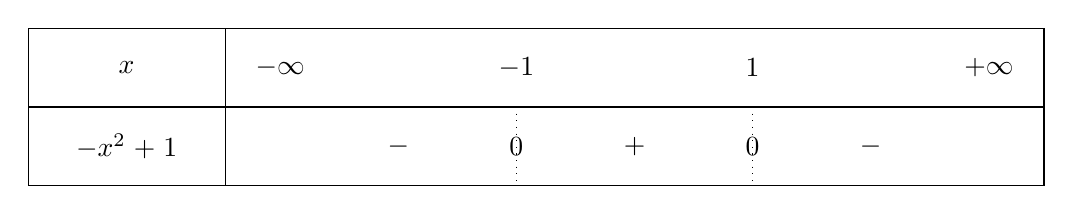
\begin{tikzpicture}
   \tkzTabInit[lgt = 2.5, espcl = 3, deltacl = 0.7]{$x$ / 1 , $-x^2 + 1$ / 1 }{$-\infty$, $-1$,$1$, $+\infty$}
   \tkzTabLine{,-,z,+,z,-,}
\end{tikzpicture}

Sur $]-\infty ; -1] \cup [1;+\infty[$ $g'(x) \leq 0$ donc g est décroissant

Sur $[-1 ; 1]$ $g'(x) \geq 0$ donc g est croissant

\textbf{Limites}

$
\begin{aligned}
\lim\limits_{x \to -\infty}g(x)&=\lim\limits_{x \to -\infty}-x^3 + 3x - 4\\
                               &=\lim\limits_{x \to -\infty}-x^3\\
                               &=+\infty										
\end{aligned}
$

$
\begin{aligned}
\lim\limits_{x \to +\infty}g(x)&=\lim\limits_{x \to +\infty}-x^3 + 3x - 4\\
                               &=\lim\limits_{x \to +\infty}-x^3\\
                               &=-\infty										
\end{aligned}
$

$
\begin{aligned}
g(-1) &= -(-1)^3 + 3(-1) - 4\\
g(-1) &= 1 -3 - 4\\
      &=-6							
\end{aligned}
$

$
\begin{aligned}
g(1) &= -(1)^3 + 3(1) - 4\\
g(1) &= -1 +3 - 4\\
      &=-2							
\end{aligned}
$

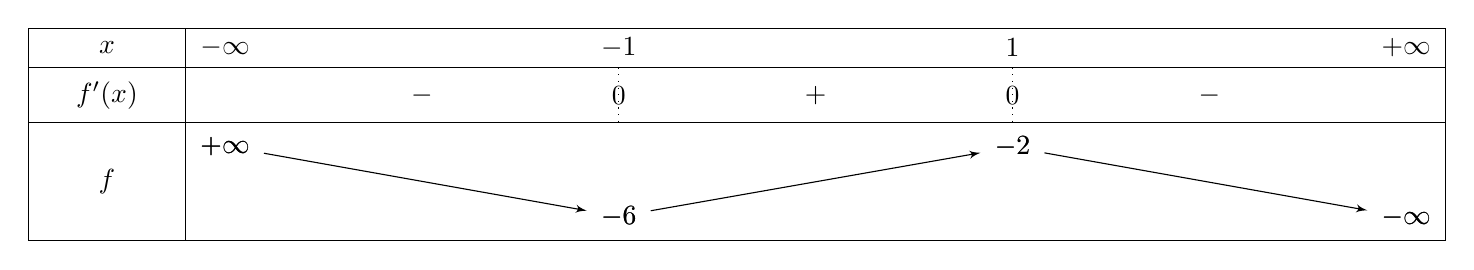
\begin{tikzpicture}[node style/.style={fill opacity=0,text opacity=1}]
        \tkzTabInit[espcl=5]{$x$/.5,$f'(x)$/.7,$f$/1.5}{$-\infty$,$-1$,$1$,$+\infty$}
        \tkzTabLine{,-,z,+,z,-,}
        \tkzTabVar{+/$+\infty$,-/$-6$,+/$-2$,-/$-\infty$/}
        %\tkzTabVal[draw]{1}{2}{0.3}{$0$}{$0$}
\end{tikzpicture}       
    
    \item 
    \begin{enumerate}
        \item Montrons que l'équation $g(x)=0$ admet une unique solution $\alpha \in \mathbb{R}$. \textbf{(0,5pt)}

\underline{\textbf{Existance}}

D'après le tableau de vairation $\lim\limits_{x \to -\infty}g(x) \times g(-1) < 0 $ d'où l'existance d'une solution

\underline{\textbf{Unicité}}

$g$ est continue et strictement décroissant de $]-\infty , -1[$ vers $]+\infty , -6[$ d'où l'unicité de la solution      
        
        \item Donnons un encadrement de $\alpha$ à $10^{-1}$. \textbf{(0,5pt)}

On sait que la solution unique $\alpha$ vérifie $\alpha<-1$.

Calculons $g(x)=-x^3+3x-4$ pour deux valeurs décimales consécutives.

\[
g(-2)= -(-8)+3(-2)-4 = 8-6-4 = -2 < 0
\]

\[
g(-1{,}5)= -(-3{,}375)+3(-1{,}5)-4 = 3{,}375-4{,}5-4 = -5{,}125 < 0
\]

On cherche donc plus à gauche.

\[
g(-2{,}1)= -(-9{,}261)+3(-2{,}1)-4 = 9{,}261-6{,}3-4 = -1{,}039 < 0
\]

\[
g(-2{,}2)= -(-10{,}648)+3(-2{,}2)-4 = 10{,}648-6{,}6-4 = 0{,}048 > 0
\]

La fonction $g$ est continue et strictement décroissante sur $]-\infty,-1]$, donc elle change de signe une seule fois sur cet intervalle.

\bigskip

\textbf{Encadrement à $10^{-1}$ :}

\[
\boxed{-2{,}2 < \alpha < -2{,}1}
\]
        
        
    \end{enumerate}
    \item En déduire le signe de $g(x)$ sur $]-\infty; 0]$. \textbf{(0,25pt)}

\[
\begin{array}{ll}
g(x)>0 & \text{si } x\in ]-\infty,\alpha[ \\
g(x)=0 & \text{si } x=\alpha \\
g(x)<0 & \text{si } x\in ]\alpha,0]
\end{array}
\]    
    
\end{enumerate}

\hrule
\vskip 0.5cm

% --- Partie B ---
\underline{\textbf{Partie B : Étude de la fonction $f$}} \textcolor{red}{\textbf{(9pts)}}
\begin{enumerate}
    \item Déterminons l'ensemble de définition $D_f$ de $f$. \textbf{(0,5pt)}

$$
\begin{aligned}
f(x) =
\begin{cases}
\dfrac{x^3 - 2x^2}{x^2 - 1} & \text{; si } x \leq 0 \\
x + \sqrt{x^2 + x} & \text{; si } x > 0
\end{cases} \text{ Posons }
f(x) =
\begin{cases}
f_{1}(x) & \text{; si } x \leq 0 \\
f_{2}(x) & \text{; si } x > 0
\end{cases}
\end{aligned}
$$    

\begin{itemize}
\item $f_{1}$

$
\begin{aligned}
f_{1} \quad \exists \quad \text{ ssi } & x^2 - 1 \neq 0 \text{ et } x \leq 0\\
												 & x \neq -1 \text{ et } x \neq -1 \text{ et } x \in ]-\infty,0] \\
												 & -1 \in ]-\infty,0] \text{ et }  1  \notin ]-\infty,0] \\
\end{aligned}
$	

$$\underline{Df_{1} = ]-\infty ; -1[ \cap ]-1 ; 0[}$$

\item $f_{2}$

$ f_{2} \quad \exists \quad$ ssi  $x^2 + x \geq 0 $ et $x > 0$

Posons $x^2 + x = 0 $

$x^2 + x = 0  \implies x=0 \textbf{ ou } x=-1$       
   
    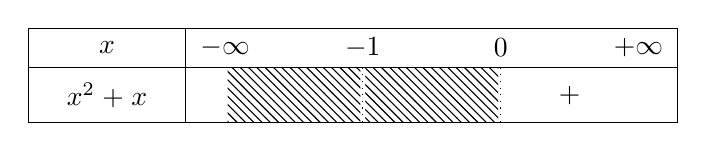
\begin{tikzpicture}[node style/.style={fill opacity=0,text opacity=1}]
        \tkzTabInit[espcl=1.75]{$x$/.5,$x^2 + x$/.7}{$-\infty$,$-1$,$0$,$+\infty$}
        \tkzTabLine{, h, t, h, t, +, }
    \end{tikzpicture}
    
    \underline{$Df_{2} = ]0 ; +\infty[$}  
\end{itemize}

$$ \text{Donc}\quad
\begin{aligned}
Df & = Df_{1} \cup Df_{2} \\
    & = ]-\infty ; -1[ \cap ]-1 ; 0[ \cup ]0 ; +\infty[\\
    &=\mathbb{R}\setminus \{-1\}
\end{aligned}
$$
    
    \begin{resultbox}
    \[
    \mathbf{Df = \mathbb{R}\setminus \{-1\} }
    \]
   \end{resultbox} 
   
    \item 
    \begin{enumerate}
    	\item
					\begin{itemize}
						\item Calculons les limites de $f$ aux bornes de $D_f$ . \textbf{(1pt)}

							\begin{itemize}
									\item \underline{En $-\infty$}: $f(x)=f_{1}(x)$   
    
\(
\begin{aligned}
 \lim\limits_{x \to -\infty} f(x) &= \lim\limits_{x \to -\infty} \dfrac{x^3 - 2x^2}{x^2 - 1}\\
 																	&= \lim\limits_{x \to -\infty} \dfrac{x^3}{x^{2}}\\
 																	&= \lim\limits_{x \to -\infty} x\\
 																	&= -\infty
\end{aligned}    
\)

    \begin{resultbox}
    \[
    \mathbf{\lim\limits_{x \to -\infty} f(x) = -\infty }
    \]
   \end{resultbox}

									\item \underline{En $+\infty$}: $f(x)=f_{2}(x)$   
    
\(
\begin{aligned}
 \lim\limits_{x \to +\infty} f(x) &= \lim\limits_{x \to +\infty} x + \sqrt{x^2+x}\\
 																	&= \lim\limits_{x \to +\infty} x + \sqrt{x^2+x}\\
 																	&= +\infty
\end{aligned}    
\)

    \begin{resultbox}
    \[
    \mathbf{\lim\limits_{x \to +\infty} f(x) = +\infty }
    \]
   \end{resultbox}

									\item \underline{En $-1^{-}$}: $f(x)=f_{1}(x)$

\(
\begin{aligned}
 \lim\limits_{x \to -1^{-}} f(x) &= \lim\limits_{x \to 1^{-}} \dfrac{x^3 - 2x^2}{x^2 - 1}\\
 																	&=  "\dfrac{-3}{0}"
 		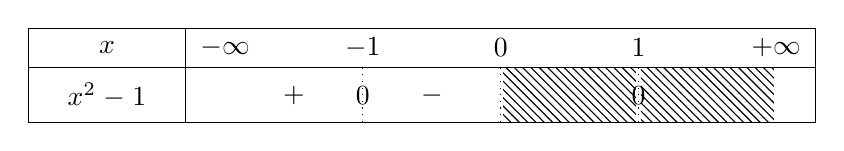
\begin{tikzpicture}[node style/.style={fill opacity=0,text opacity=1}]
        \tkzTabInit[espcl=1.75]{$x$/.5,$x^2 - 1$/.7}{$-\infty$,$-1$,$0$,$1$,$+\infty$}
        \tkzTabLine{, +, z, -, t,h, z, h,}
    \end{tikzpicture}\\
 																	&=  "\dfrac{-3}{0^{+}}"\\
 																	&= -\infty
\end{aligned}    
\)

    \begin{resultbox}
    \[
    \mathbf{\lim\limits_{x \to -1^{-}} f(x) =-\infty }
    \]
   \end{resultbox}

										\item \underline{En $-1^{+}$}: $f(x)=f_{1}(x)$

\(
\begin{aligned}
 \lim\limits_{x \to -1^{+}} f(x) &= \lim\limits_{x \to 1^{+}} \dfrac{x^3 - 2x^2}{x^2 - 1}\\
 																	&= \dfrac{-3}{0^{-}}\\
 																	&= +\infty
\end{aligned}    
\)

    \begin{resultbox}
    \[
    \mathbf{\lim\limits_{x \to -1^{+}} f(x) =+\infty }
    \]
   \end{resultbox}
   								\end{itemize}
\item Déduisons-en l'existence d'une asymptote dont on précisera.\textbf{(0,25pt)}

Comme $\lim\limits_{x \to -1} f(x) = \infty$ donc $x=-1$ est une asymptote verticale

    \begin{resultbox}
    \[
    \mathbf{ \text{Donc }   x = -1  \text{ est une asymptote verticale à } (\mathcal{C}_f) }
    \]
   \end{resultbox}

  \end{itemize}     
        \item 
        \begin{itemize}
        \item Pour $x \leq 0$, déterminons les réels $a, b, c$ et $d$ tels que : 
        $f(x)=ax+b+\dfrac{cx+d}{x^2-1}$\textbf{(0,5pt)}

 $
 \begin{aligned}  
 f(x)=ax+b+\dfrac{cx+d}{x^2-1} &\implies f(x)=\frac{(ax+b)(x^2-1)+cx+d}{x^2-1}\\
                               &\implies f(x)=\frac{ax^3+bx^2-ax-b+cx+d}{x^2-1}\\
                               &\implies f(x)=\frac{ax^3+bx^2+(c-a)x+(d-b)}{x^2-1}
 \end{aligned} 
 $   

On a $\dfrac{x^3 - 2x^2}{x^2 - 1}=\frac{ax^3+bx^2+(c-a)x+(d-b)}{x^2-1}$ 

par identification  
$
 \begin{aligned}  
	\begin{cases} 
	a = 1\\
	b = -2\\
	c-a = 0\\
	d-b = 0
	\end{cases}
	&\implies
		\begin{cases} 
	a = 1\\
	b = -2\\
	c-1 = 0\\
	d+2 = 0
	\end{cases}
		&\implies
		\begin{cases} 
	a = 1\\
	b = -2\\
	c= 1\\
	d = -2
	\end{cases}
 \end{aligned} 
 $ 

Ainsi, $f(x)=x-2+\dfrac{x-2}{x^2-1}$   
         
        \item Déduisons-en la nature de la branche infinie en $-\infty$. \textbf{(0,25pt)}

En posant $(\Delta_1):  y = x -2$, si $ \lim\limits_{x \to -\infty} f(x) - y = 0 $ alors $y=x-2$ est asymptote oblique

En effet 

\(
\begin{aligned}
 \lim\limits_{x \to -\infty} f(x) - y &= \lim\limits_{x \to -\infty}\dfrac{x-2}{x^2-1} \\
 																	&= \lim\limits_{x \to -\infty} \dfrac{x}{x^2}\\
 																	&= 0\\
\end{aligned}    
\)        

    \begin{resultbox}
    \[
    \mathbf{ \text{Donc } (\Delta_1):  y = x -2 \text{ est une asymptote oblique à } (\mathcal{C}_f) \text{en } -\infty }
    \]
   \end{resultbox}      
        
 %Autre méthode
\begin{comment}
 Comme $\lim\limits_{x \to -\infty} f(x) = +\infty$  

\begin{itemize}
\item Cherchons  $\lim\limits_{x \to -\infty} \dfrac{f(x)}{x} $  

\(
\begin{aligned}
 \lim\limits_{x \to -\infty} \dfrac{f(x)}{x} &= \lim\limits_{x \to -\infty} \dfrac{\dfrac{x^3 - 2x^2}{x^2 - 1}}{x}\\
 																	&= \lim\limits_{x \to -\infty} \dfrac{x^3 - 2x^2}{x^3 - x}\\
 																	&= \lim\limits_{x \to -\infty} \dfrac{x^2}{x^3}\\
 																	&= 1
\end{aligned}    
\)        

Donc  $\lim\limits_{x \to -\infty} \dfrac{f(x)}{x} = 1 $       

\item Cherchons  $\lim\limits_{x \to -\infty} f(x)-x $ 

\(
\begin{aligned}
 \lim\limits_{x \to -\infty} f(x)-x &= \lim\limits_{x \to -\infty} \dfrac{x^3 - 2x^2}{x^2 - 1}-x\\
 																	&= \lim\limits_{x \to -\infty} \dfrac{x^3-2x^{2}-x^3+x}{x^2 - 1}\\
 																	&= \lim\limits_{x \to -\infty} \dfrac{-2x^{2}}{x^{2}}\\
 																	&= -2
\end{aligned}    
\) 

\end{itemize}

    \begin{resultbox}
    \[
    \mathbf{ \text{Donc } (\Delta_1):  y = x -2 \text{ est une asymptote oblique à } (\mathcal{C}_f) \text{en } -\infty }
    \]
   \end{resultbox}
\end{comment}
%Autre méthode
        \end{itemize}
        
        \item Donner la nature de l'asymptote en $+\infty$. \textbf{(0,5pt)}

Comme $\lim\limits_{x \to +\infty} f(x) = -\infty$ 

\begin{itemize}
\item Cherchons  $\lim\limits_{x \to +\infty} \dfrac{f(x)}{x} $  

\(
\begin{aligned}
 \lim\limits_{x \to +\infty} \dfrac{f(x)}{x} &= \lim\limits_{x \to +\infty}  \dfrac{x + \sqrt{x^2+x}}{x}\\
 																	&= \lim\limits_{x \to +\infty} \dfrac{x\left(1 + \sqrt{1+\dfrac{1}{x}}\right)}{x}\\
 																	&= \lim\limits_{x \to +\infty} \left(1 + \sqrt{1+\dfrac{1}{x}}\right)\\
 																	&= 2
\end{aligned}    
\)        

Donc  $\lim\limits_{x \to +\infty} \dfrac{f(x)}{x} = 2 $       

\item Cherchons  $\lim\limits_{x \to +\infty} f(x)-2x $ 

\(
\begin{aligned}
 \lim\limits_{x \to +\infty} f(x)-2x &= \lim\limits_{x \to +\infty} x + \sqrt{x^2+x}-2x\\
 																		 &= \lim\limits_{x \to +\infty} \sqrt{x^2+x}-x\\
 																		 &= \lim\limits_{x \to +\infty} \dfrac{x^2+x-x^2}{\sqrt{x^2+x}+x} \\
 																		 &= \lim\limits_{x \to +\infty} \dfrac{x}{\sqrt{x^2+x}+x} \\
 																		 &= \lim\limits_{x \to +\infty} \dfrac{x}{x\left(1 + \sqrt{1+\dfrac{1}{x}}\right)} \\
 																		 &= \lim\limits_{x \to +\infty} \dfrac{1}{\left(1 + \sqrt{1+\dfrac{1}{x}}\right)} \\
 																	   &= \dfrac{1}{2}
\end{aligned}    
\)   
 
\end{itemize}
  		    
    \begin{resultbox}
    \[
    \mathbf{ \text{Donc } (\Delta_2):  y = 2x+\dfrac{1}{2}  \text{ est une asymptote oblique à } (\mathcal{C}_f) \text{en } +\infty }
    \]
   \end{resultbox}         
        
    \end{enumerate}
    \item 
    \begin{enumerate}
        \item Montrons que $f$ est continue sur $D_f$. \textbf{(0,75pt)}

\begin{itemize}
\item \textbf{Continuité sur chaque intervalle}

\begin{itemize}
\item \textbf{ Sur $]-\infty,0]\setminus\{-1\}$}

La fonction
\(
x\longmapsto \dfrac{x^3-2x^2}{x^2-1}
\)est une fonction rationnelle. 

Elle est donc continue sur son domaine de définition
\(
\mathbb{R}\setminus\{-1,1\}.
\)

En particulier, elle est continue sur $]-\infty,0]\setminus\{-1\}$.

\medskip

\item \textbf{ Sur $]0,+\infty[$}

Pour tout $x>0$, on a $x^2+x>0$, donc la fonction
\(
x\longmapsto \sqrt{x^2+x}
\)
est bien définie et continue sur $]0,+\infty[$.

Ainsi, la fonction
\(
x\longmapsto x+\sqrt{x^2+x}
\)
étant somme de fonctions continues, est continue sur $]0,+\infty[$.
\end{itemize}

\item \textbf{ Continuité en $0$}

 \begin{itemize}
\item \underline{En $0^-$}: $f(x)=f_{1}(x)$   
    
\(
\begin{aligned}
 \lim\limits_{x \to 0^-} f(x) &= \lim\limits_{x \to 0^-} \dfrac{x^3-2x^2}{x^2-1}\\
 															&= 0
\end{aligned}    
\)

\textcolor{red}{{\underline{$\lim\limits_{x \to 0^-} f(x) = 0$}}}

\item \underline{En $0^+$}: $f(x)=f_{2}(x)$   
    
\(
\begin{aligned}
 \lim\limits_{x \to 0^+} f(x) &= \lim\limits_{x \to 0^+} \bigl(x+\sqrt{x^2+x}\bigr)\\
															&=0
\end{aligned}    
\)

\textcolor{red}{{\underline{$\lim\limits_{x \to 0^+} f(x) = 0$}}}
\end{itemize}   

On a $f(0)=\dfrac{0^3-2\cdot 0^2}{0^2-1}=0$

\textcolor{red}{Finalement $\lim\limits_{x \to 0^-} f(x) = \lim\limits_{x \to 0^+} f(x) = f(0)$ donc f est continue en $0$}

\item \textbf{ Conclusion}

La fonction $f$ est continue sur $]-\infty,0]\setminus\{-1\}$, sur $]0,+\infty[$ et en $0$.

    \begin{resultbox}
    \[
    \mathbf{ \lim\limits_{x \to 0^-} f(x) = \lim\limits_{x \to 0^+} f(x) = f(0)=0 \text{ donc } f \text{ est continue sur } D_f=\mathbb{R}\setminus\{-1\}. }
    \]
   \end{resultbox} 

\end{itemize}       
        
        \item Étudions la dérivabilité de $f$ en $0$ puis interprétons le résultat obtenu. \textbf{(1,5pt)}

\begin{itemize}
\item Étudions la dérivabilité de $f$ en $0$
\begin{itemize}
\item \underline{En $0^-$}: $f(x)=f_{1}(x)$ 

\(
\begin{aligned}
 \lim\limits_{x \to 0^-} \dfrac{f(x)-f(0)}{x} &= \lim\limits_{x \to 0^-} \dfrac{\dfrac{x^3-2x^2}{x^2-1}}{x}\\
 															                &= \lim\limits_{x \to 0^-} \dfrac{x^3-2x^2}{x^2-x}\\
 															                &= \lim\limits_{x \to 0^-} \dfrac{x^2-2x}{x-1}\\
 															                &=0
\end{aligned}    
\)

\item \underline{En $0^+$}: $f(x)=f_{2}(x)$ 

\(
\begin{aligned}
\lim\limits_{x \to 0^+} \dfrac{f(x)-f(0)}{x} &=\lim\limits_{x \to 0^+} \dfrac{x + \sqrt{x^2+x}}{x}\\
															               &=\lim\limits_{x \to 0^+} \dfrac{x^2-x^2-x}{x(x - \sqrt{x^2+x})}\\
															               &=\lim\limits_{x \to 0^+} \dfrac{-x}{x(x - \sqrt{x^2+x})}\\
															               &=\lim\limits_{x \to 0^+} \dfrac{-1}{(x - \sqrt{x^2+x})}\\
															               &="\dfrac{-1}{0}"\\
\end{aligned}    
\)

Supposons que $ x - \sqrt{x^2+x} > 0 $

$ x - \sqrt{x^2+x} > 0 \implies \sqrt{x^2+x} < x $

$
\begin{aligned}
\sqrt{x^2+x} < x &\implies \begin{cases}
										x^2+x > 0\\
										x > 0\\ 
										x^2+x < x^{2} 
										\end{cases}\\
									&\implies \begin{cases}
										x^2+x > 0\\
										x > 0\\ 
										x < 0
										\end{cases}\\
\end{aligned}
$

$
\begin{aligned}
\begin{cases}
x^2+x = 0\\
x = 0 
\end{cases}\implies
\begin{cases}
x=0 \textbf{ ou } x=-1\\
x = 0
\end{cases}
\end{aligned}
$

    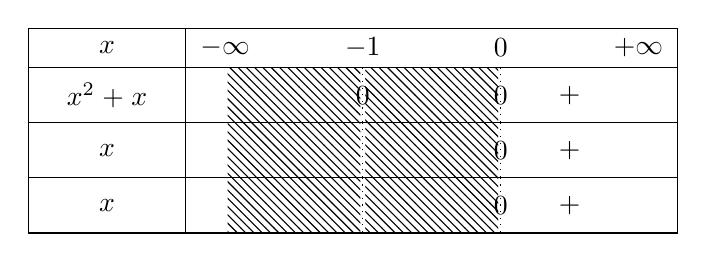
\begin{tikzpicture}[node style/.style={fill opacity=0,text opacity=1}]
        \tkzTabInit[espcl=1.75]{$x$/.5,$x^2 + x$/.7,$x$/.7,$x$/.7}{$-\infty$,$-1$,$0$,$+\infty$}
        \tkzTabLine{,h,z,h,z,+, }
        \tkzTabLine{,h,t,h,z,+, }
        \tkzTabLine{,h,t,h,z,+, }
    \end{tikzpicture}

$$ S = \emptyset $$ Ainsi, il n'existe pas de $ x > 0 $ pour lequel $ x-\sqrt{x^2+x} > 0  $

 $$ \textbf{Donc } x-\sqrt{x^2+x} <0,  \, \forall x\in ]0;+\infty[ $$

\textcolor{red}{Ainsi  $\forall x\in ]0;+\infty[$ $f'(x) > 0 $ donc f  est croissant $0;+\infty[$}

\(
\begin{aligned}
\lim\limits_{x \to 0^+} \dfrac{f(x)-f(0)}{x} &=\lim\limits_{x \to 0^+} \dfrac{-1}{(x - \sqrt{x^2+x})}\\
															               &=\dfrac{-1}{0^-}\\
															               &=+\infty \\
\end{aligned}    
\)

\textcolor{red}{ Autre Méthode }

+++++++++++++++++++++++++++++++++++++++++++++

On calcule la dérivée à droite en $0$ :
\[
f'_+(0)=\lim_{x\to 0^+}\frac{f(x)-f(0)}{x}
=\lim_{x\to 0^+}\frac{x+\sqrt{x^2+x}}{x}.
\]

On écrit :
\[
\frac{x+\sqrt{x^2+x}}{x}
=1+\frac{\sqrt{x^2+x}}{x}.
\]

Or,
\[
\frac{\sqrt{x^2+x}}{x}
=\sqrt{\frac{x^2+x}{x^2}}
=\sqrt{1+\frac{1}{x}}.
\]

Lorsque $x\to 0^+$, on a $\dfrac{1}{x}\to +\infty$, donc
\[
\sqrt{1+\frac{1}{x}}\to +\infty.
\]

Ainsi,
\[
f'_+(0)=+\infty.
\]

++++++++++++++++++++++++++++++++++++++++++++++++

    \begin{resultbox}
    \[
    \mathbf{ \lim\limits_{x \to 0^+} \dfrac{f(x)-f(0)}{x} = 0 \text{ et } \lim\limits_{x \to 0^+} \dfrac{f(x)-f(0)}{x} = +\infty }
    \]
   \end{resultbox} 

\end{itemize}  
\item Interprétons le résultat obtenu.

\begin{itemize}
\item \textcolor{red}{ $f$ est dérivable à gauche de $0$ et $y=2x$ est une démi-tangent en $0^-$ } ;
\item \textcolor{red}{ $f$ n'est pas dérivable à droite de $0$ donc admet une démi-tangent orientée vers le haut en $0^+$  }
\end{itemize}
Le point d’abscisse $0$ est donc un point anguleux, ce qui explique la non-dérivabilité de $f$ en $0$.
\end{itemize}        

\begin{comment} %Autre méthode
\subsubsection*{1. Dérivée à gauche en $0$}

On calcule la dérivée à gauche en $0$ :
\[
f'_-(0)=\lim_{x\to 0^-}\frac{f(x)-f(0)}{x-0}
=\lim_{x\to 0^-}\frac{\dfrac{x^3-2x^2}{x^2-1}}{x}.
\]

Ainsi,
\[
f'_-(0)=\lim_{x\to 0^-}\frac{x^3-2x^2}{x(x^2-1)}
=\lim_{x\to 0^-}\frac{x(x-2)}{x^2-1}.
\]

En faisant tendre $x$ vers $0$, on obtient :
\[
f'_-(0)=\frac{0\cdot(-2)}{-1}=0.
\]

\subsubsection*{2. Dérivée à droite en $0$}

On calcule la dérivée à droite en $0$ :
\[
f'_+(0)=\lim_{x\to 0^+}\frac{f(x)-f(0)}{x}
=\lim_{x\to 0^+}\frac{x+\sqrt{x^2+x}}{x}.
\]

On écrit :
\[
\frac{x+\sqrt{x^2+x}}{x}
=1+\frac{\sqrt{x^2+x}}{x}.
\]

Or,
\[
\frac{\sqrt{x^2+x}}{x}
=\sqrt{\frac{x^2+x}{x^2}}
=\sqrt{1+\frac{1}{x}}.
\]

Lorsque $x\to 0^+$, on a $\dfrac{1}{x}\to +\infty$, donc
\[
\sqrt{1+\frac{1}{x}}\to +\infty.
\]

Ainsi,
\[
f'_+(0)=+\infty.
\]

\subsubsection*{3. Conclusion}

La dérivée à gauche en $0$ est finie :
\[
f'_-(0)=0,
\]
tandis que la dérivée à droite est infinie :
\[
f'_+(0)=+\infty.
\]

Par conséquent,
\[
\boxed{f \text{ n’est pas dérivable en } 0.}
\]

\subsubsection*{4. Interprétation graphique}

La courbe représentative de $f$ admet :
\begin{itemize}
\item à gauche de $0$, une tangente horizontale ;
\item à droite de $0$, une tangente verticale.
\end{itemize}

Le point d’abscisse $0$ est donc un point anguleux, ce qui explique la non-dérivabilité de $f$ en $0$.  
\end{comment}      
        
    \end{enumerate}
    \item Démontrons que : $ f(x) = -2+\dfrac{3(\alpha-2)}{\alpha^2 - 1} $. \textbf{(0,5pt)}

   $f(x) = \dfrac{x^3 - 2x^2}{x^2 - 1} \implies f(x) = \dfrac{\alpha^3 - 2\alpha^2}{\alpha^2 - 1} $    

	Comme  $g(\alpha) = 0 $ alos $ -\alpha^3 + 3\alpha - 4 = 0$ donc $\alpha^3 = 3\alpha - 4$

 Ainsi, 
 
 \(
 \begin{aligned} 
 f(\alpha) = \dfrac{\alpha^3 - 2\alpha^2}{\alpha^2 - 1} &\implies f(\alpha) = \dfrac{\alpha^3 - 2\alpha^2}{\alpha^2 - 1}\\
 &\implies f(\alpha) = \dfrac{3\alpha - 4 - 2\alpha^2}{\alpha^2 - 1}\\  
 &\implies f(\alpha) = -\dfrac{2\alpha^2-3\alpha+4}{\alpha^2 - 1}\\
 &\implies f(\alpha) = -\dfrac{2(\alpha^2-1)-3(\alpha-2)}{\alpha^2 - 1}\\   
 &\implies f(\alpha) = \dfrac{-2(\alpha^2-1)+3(\alpha-2)}{\alpha^2 - 1}\\
 &\implies f(\alpha) = \dfrac{-2(\alpha^2-1)}{\alpha^2 - 1}+\dfrac{3(\alpha-2)}{\alpha^2 - 1}\\
  &\implies f(\alpha) = -2+\dfrac{3(\alpha-2)}{\alpha^2 - 1}\\
 \end{aligned}    
 \)      
    
    \item 
    \begin{enumerate}
        \item Montrons que $\forall x \in ]-\infty; -1[ \cup ]-1; 0[$, on a : 
        $f'(x) = \dfrac{-xg(x)}{(x^2-1)^2}$ puis étudier son signe
\begin{itemize}
\item Montrons que $\forall x \in ]-\infty; -1[ \cup ]-1; 0[$, on a : 
        $f'(x) = \dfrac{-xg(x)}{(x^2-1)^2}$ \textbf{(0,5pt)}
        
On a : $ f'(x)=\dfrac{-xg(x)}{(x^2-1)^2} $

La fonction $f$ est dérivable sur $]-\infty,-1[ \cup ]-1,0[$ comme quotient de fonctions dérivables,
avec $x^2-1\neq 0$ sur ces intervalles.

\(
 \begin{aligned} 
 f'(x) &= \dfrac{(x^3-2x^2)'(x^2-1)-(x^3-2x^2)(x^2-1)'}{(x^2-1)^2}\\
       &= \dfrac{(3x^2-4x)(x^2-1)-(x^3-2x^2)(2x)}{(x^2-1)^2}.\\
       &= \dfrac{3x^4-3x^2-4x^3+4x-(2x^4-4x^3)}{(x^2-1)^2}\\
       &= \dfrac{x^4-3x^2+4x}{(x^2-1)^2}\\
       &= \dfrac{-x(-x^3+3x-4)}{(x^2-1)^2}\\
       &=\dfrac{-xg(x)}{(x^2-1)^2}
 \end{aligned}    
 \)  

Ainsi,
\(
\forall x \in ]-\infty,-1[ \cup ]-1,0[, \quad
f'(x)=\dfrac{-xg(x)}{(x^2-1)^2}.
\)   

\item le signe de $f'(x)$ dépend du numérateur \textbf{(0,5pt)}    

    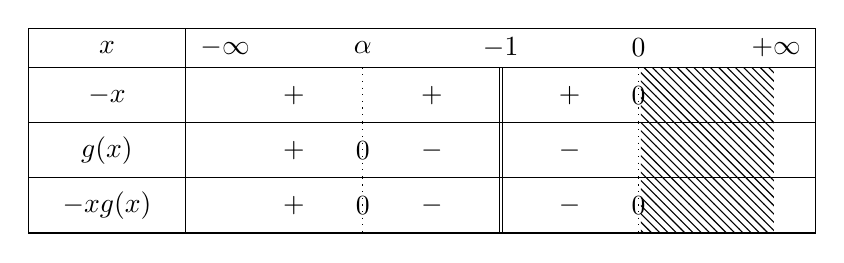
\begin{tikzpicture}[node style/.style={fill opacity=0,text opacity=1}]
        \tkzTabInit[espcl=1.75]{$x$/.5,$-x$/.7,$g(x)$/.7,$-xg(x)$/.7}{$-\infty$,$\alpha$,$-1$,$0$,$+\infty$}
        \tkzTabLine{, +, t,+,d ,+, z,h, }
        \tkzTabLine{, +, z,-,d ,-, t,h, }
        \tkzTabLine{, +, z,-,d ,-, z,h, }
    \end{tikzpicture}    

Ansi, 
 
\textcolor{red}{ si \(x\in ]-\infty,\alpha]\,, f'(x) \geq 0 \)  donc f est croissante sur $]-\infty; \alpha]$}  

\textcolor{red}{ si \(x\in [\alpha,-1[ \cup]-1,0] \,, f'(x) \leq 0 \)  donc f est croissante sur $[\alpha,-1[ \cup]-1,0]$}  

\end{itemize}  
        \item Calculons $f'(x)$ sur $]0; +\infty[$ et étudions son signe.

			\begin{itemize}
			\item Calculons $f'(x)$ sur $]0; +\infty[$ \textbf{(0,5pt)}
			
\(
\begin{aligned}
f'(x) &= 1 + \dfrac{2x+1}{2\sqrt{x^2+x}}\\
      &= \dfrac{2\sqrt{x^2+x}+2x+1}{2\sqrt{x^2+x}}\\
      &= \dfrac{2\sqrt{x^2+x}+2x+1}{2\sqrt{x^2+x}} \\
\end{aligned}
\)

			\item étudions son signe \textbf{(0,25pt)}

 Si $ x>0\,, f'(x)= \dfrac{2\sqrt{x^2+x}+2x+1}{2\sqrt{x^2+x}}$ le signe dépend du numérateur 			

$$ \textbf{Or } 2\sqrt{x^2+x}+2x+1 > 0 \, \forall x\in ]0;+\infty[ $$

\textcolor{red}{Ainsi  $\forall x\in ]0;+\infty[$ $f'(x) > 0 $ donc f  est croissant $]0;+\infty[$}		
			
			\end{itemize}			        
        
        \item Dressons le tableau de variation de $f$ sur $D_f$. \textbf{(0,75pt)}

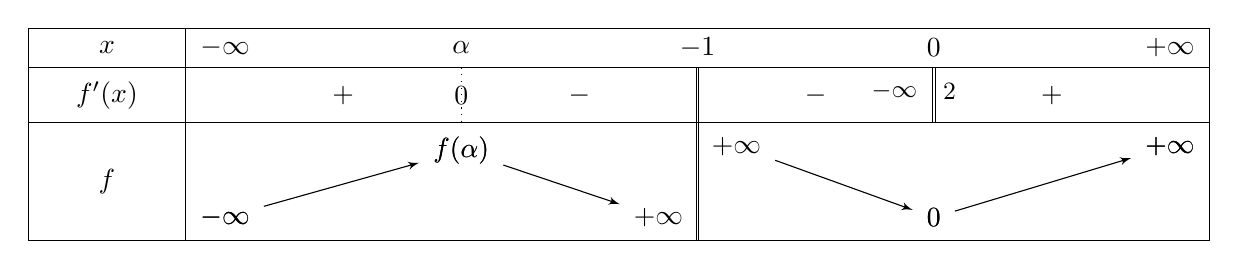
\begin{tikzpicture}[node style/.style={fill opacity=0,text opacity=1}]
        \tkzTabInit[espcl=3]{$x$/.5,$f'(x)$/.7,$f$/1.5}{$-\infty$,$\alpha$,$-1$,$0$,$+\infty$}
        \tkzTabLine{,+,z,-,d,-,d,+,}
        \tkzTabVar{-/$-\infty$,+/$f(\alpha)$,-D+/ $+\infty$, -/$0$,+/$+\infty$/}
        \node at (11,-0.8) {\small $-\infty$};
        \node at (11.7,-0.8) {\small $2$};
\end{tikzpicture}          
        
    \end{enumerate}
    \item Construisons soigneusement la courbe $(C_f)$. \textbf{(0,75 pt)}
\end{enumerate}

\begin{center}
\begin{figure}[H]% Forcer l'image à cet endroit
\centering
\includegraphics[width=0.8\textwidth]{devoir2-2025-2026.png}
\caption{Courbe de (Cf)}
\label{fig:monimage}
\end{figure}
\href{https://www.geogebra.org/classic/q97sf6ew}{Clique ici pour voir la courbe sur géogébra}
\end{center}

\underline{\textbf{Partie C : Bijection}} \textcolor{red}{\textbf{(1,75pts)}}

Soit $h$ la restriction de $f$ sur $I = ]0; +\infty[$.
\begin{enumerate}
    \item Montrons que $h$ réalise une bijection de $I$ vers un intervalle $J$ à préciser. \textbf{(0,25pt)}

Sur $I$ $h$ est continue est strictement croissante donc réalise une bijection de $I$ vers $J=[0,+\infty[$

		Comme $\forall x \in I$, $h'(x)\neq 0$ donc $h^{-1}$ est dérivable sur $J$    
    
    \item Calculons $h^{-1}(1)$ et $(h^{-1})'(\sqrt{2}+1)$. \textbf{(0,5pt)}

\(
h(x)=x+\sqrt{x^2+x}.
\)

\begin{itemize}

\item  \textbf{ Calcul de $h(1)$}

$h(1) = \sqrt{2}+1$ 

\begin{resultbox}
    \[
        \mathbf{ h(1) = \sqrt{2}+1 }
    \]
\end{resultbox} 

\item  \textbf{ Calcul de $(h^{-1})'(\sqrt{2}+1)$}

\(
(h^{-1})'(\sqrt{2}+1)=\dfrac{1}{h'(h^{-1}(\sqrt{2}+1))} \textbf{ Or } h(1) = \sqrt{2}+1 \textbf{ donc } h^{-1}(\sqrt{2}+1) = 1
\)

\(
\begin{aligned}
(h^{-1})'(\sqrt{2}+1)
&= \dfrac{1}{h'\!\left(1\right)} \textbf{ comme } h'(x)=1+\dfrac{2x+1}{2\sqrt{x^2+x}}\\
&=\dfrac{1}{1+\dfrac{2+1}{2\sqrt{1^2+1}}}\\
&=\dfrac{1}{1+\dfrac{3}{2\sqrt{2}}}\\
&=\dfrac{1}{ \dfrac{2\sqrt{2}+3}{2\sqrt{2}}}\\
&=\dfrac{2\sqrt{2}}{2\sqrt{2}+3}
\end{aligned}
\)

\begin{resultbox}
    \[
        \mathbf{(h^{-1})'(\sqrt{2}+1)=\dfrac{2\sqrt{2}}{2\sqrt{2}+3}}
    \]
\end{resultbox}  
\end{itemize}   
    
    \item Explicitons $h^{-1}(x)$. \textbf{(0,5pt)}

\[
\text{Soit } y = h(x) = x+\sqrt{x^{2}+x}.
\]

On isole la racine :
\[
y-x = \sqrt{x^{2}+x}.
\]

En élevant au carré, on obtient :
\[
(y-x)^{2} = x^{2}+x.
\]

\[
y^{2}-2xy+x^{2} = x^{2}+x.
\]

En simplifiant :
\[
y^{2}-2xy = x.
\]

On factorise par \(x\) :
\[
y^{2} = x(1+2y).
\]

D’où :

\begin{resultbox}
    \[
        \mathbf{h^{-1}(x)=\dfrac{x^{2}}{1+2x}}
    \]
\end{resultbox}    
    
    \item Construisons $(C_{h^{-1}})$ dans le repère précédent. \textbf{(0,5pt)}

\begin{center}
\begin{figure}[H]% Forcer l'image à cet endroit
\centering
\includegraphics[width=0.8\textwidth]{reciDevoir2-2025-2026}
\caption{Courbe de (Cf)}
\label{fig:monimage}
\end{figure}
\href{https://www.geogebra.org/classic/q97sf6ew}{Clique ici pour voir la courbe sur géogébra}
\end{center}    
    
\end{enumerate}

\end{document}
